\chapter{振幅调制与解调}

\section{概述}

调制:由调制信号去控制载波的三参量(振幅、频率、相位)之一,使其随调制信号线性变化。

解调:调制的逆过程,即从已调波中恢复原调制信号的过程。

调制的分类:

\begin{equation}
    \notag
    \text{调制} \left\{
        \begin{array}{l}
            \text{按调制信号} \left\{
                \begin{array}{l}
                    \text{模拟调制} \\
                    \text{数字调制}
                \end{array}
            \right. \\
            \text{按载波信号} \left\{
                \begin{array}{l}
                    \text{连续波调制} \left\{
                        \begin{array}{l}
                            \text{振幅调制 (AM)} \\
                            \text{频率调制 (FM)} \\
                            \text{相位调制 (PM)}
                        \end{array}
                    \right. \\
                    \text{脉冲波调制} \left\{
                        \begin{array}{l}
                            \text{脉冲振幅调制 (PAM)} \\
                            \text{脉冲宽度调制 (PWM)} \\
                            \text{脉冲位置调制 (PPM)} \\
                            \text{脉冲编码调制 (PCM)}
                        \end{array}
                    \right. 
                \end{array}
            \right.
        \end{array}
    \right.
\end{equation}

\section{振幅调制原理及特性}

\subsection{普通调幅波 (AM)}

设载波信号振幅为 $U_{cm}$,频率为 $\dfrac{\omega_c}{2 \pi}$,调制信号为 $u_{\Omega}(t)$,则普通调幅波信号表示为:

\begin{equation}
    u(t) = U'_m(t) \cos{\omega_c t} = \left[ U_{cm} + k_a u_{\Omega}(t) \right] \cos{\omega_c t}
\end{equation}

其中 $k_a$ 由调幅电路决定。

对于单频调制:

\begin{equation}
    u(t) = \left( U_{cm} + k_a U_{\Omega m} \cos{\Omega t} \right) \cos{\omega_c t}
    = U_{cm} \left( 1 + m_a \cos{\Omega t} \right) \cos{\omega_c t}
\end{equation}

其中 $m_a$ 称为调幅指数或调幅度,表示载波振幅受调制信号控制后改变的程度。$m_a = 0$时为未调幅;$m_a = 1$时为最大调幅;$m_a > 1$时为过量调幅,会使包络失真。通过调幅波波形计算 $m_a$ 的公式为:

\begin{equation}
    m_a = \frac{U_{m \text{max}} - U_{m \text{min}}}{U_{m \text{max}} + U_{m \text{min}}}
\end{equation}

调幅波振幅变化规律称为调幅波的包络。调幅波的包络的变化规律与调制信号波形一致。调幅波调制过程是实现频谱线性搬移的过程。

调幅波的频率分量:载波分量 $\omega_c$、上下边频分量 $\omega_c \pm \Omega$。其中载波分量不含传输信息。

调幅波的带宽:$BW = 2 \dfrac{\Omega}{2 \pi} = 2F$。

调幅波载波功率 $P_{oT} = \dfrac{1}{2} \dfrac{U_{cm}^2}{R}$;每一边频功率 $P_{\omega_c \pm \Omega} = \dfrac{1}{4} m_a^2 P_{oT}$;调幅波的平均总功率 $P_{oav} = P_{oT} \left( 1 + \dfrac{m_a^2}{2} \right)$。当 $m_a = 1$ 时,边频功率达到最大,为总功率的 $\dfrac{1}{3}$。

实际使用中,$m_a$ 在 $0.1 \sim 1$ 之间,平均值为 $0.3$。可见普通调幅波中含有信息的上下边频分量所占的功率非常小,而不含信息的载波占绝大多数,因而调幅波的功率浪费大,效率低。

\subsection{抑制载波的双边带调幅波 (DSB)}

抑制载波的双边带调幅波抑制了载波分量,只含上、下边带分量。表示为:

\begin{equation}
    u(t) = u_{\Omega}(t) u_c(t) = \left[ U_{cm} + k_a u_{\Omega}(t) \right] \cos{\omega_c t}
\end{equation}

单频调制时:

\begin{equation}
    u(t) = \frac{1}{2} U_{\Omega m } U_{cm} \left[ \cos{(\omega_c + \Omega) t} + \cos{(\omega_c - \Omega) t} \right]
\end{equation}

抑制载波的双边带调幅波包络随调制信号变化,但包络不能完全准确地反映调制信号变化规律。载波相位在调制电压零交点处突变 $180^\circ$。

\subsection{抑制载波的单边带调幅波 (SSB)}

抑制载波的单边带调幅波在单频调制时表示为:

\begin{equation}
    u(t) = \frac{1}{2} U_{\Omega m } U_{cm} \cos{(\omega_c \pm \Omega) t}
\end{equation}

抑制载波的单边带调幅波频带只有双边带调幅波的一半,频带利用率高;全部功率都含有信息,功率利用率高。

\section{振幅调制电路}

低电平调幅电路:在低功率电平时进行调制,因此它产生小功率的调幅波,然后由线性功率放大器放大,得到所要求功率的调幅波,一般用于发射机的前级。

高电平调幅电路:在所需的功率电平上进行调制,调制与功放合一,一般用于发射机的末级。一般只能产生AM。整机效率高。

\subsection{低电平调幅电路}

二极管由一个大振幅的电压源和另一个小振幅电压源共同控制,其导通和截止受大振幅电压的控制,可以近似认为二极管处于理想开关状态。

\subsubsection{单二极管开关状态调幅电路}

二极管的开关状态受大振幅电压源的控制,经带通滤波后可取出 AM 调制信号。

\begin{figure}[htbp]
    \centering
    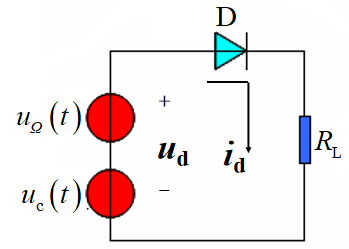
\includegraphics[scale=0.7]{image/Picture11.png}
    \caption{单二极管开关状态调幅电路}
\end{figure}

流过二极管的电流:

\begin{equation}
    i_d = \frac{1}{r_d + R_L} K(\omega_c t) u_d 
    = \left\{
        \begin{aligned}
            & \frac{1}{r_d + R_L} u_d & u_c(t) > 0 \\
            & 0 & u_c(t) < 0
        \end{aligned}
    \right.
\end{equation}

$i_d$ 中的频率成分:$(2n - 1)\omega_c \pm \Omega$、$2n \omega_c$、$\omega_c$、$\Omega$、直流分量。

\subsubsection{二极管平衡调幅电路}

$D_1$、$D_2$ 都是在 $u_c(t)$ 的正半周导通,负半周截止。经带通滤波后可取出 $\omega_c \pm \Omega$,实现 DSB 调制。

\begin{figure}[htbp]
    \centering
    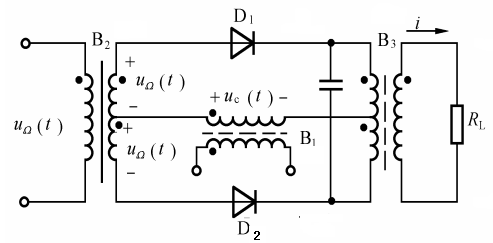
\includegraphics[scale=0.6]{image/Picture12.png}
    \caption{二极管平衡调幅电路}
\end{figure}

\subsubsection{二极管环型调幅电路}

在平衡电路的基础上,再增加两个二极管 $D_3$、$D_4$。电路中四个二极管首尾相接。$D_3$、$D_4$ 在 $u_c(t)$ 的负半周导通,正半周截止。经带通滤波后可取出 $\omega_c \pm \Omega$,实现 DSB 调制。

\begin{figure}[htbp]
    \centering
    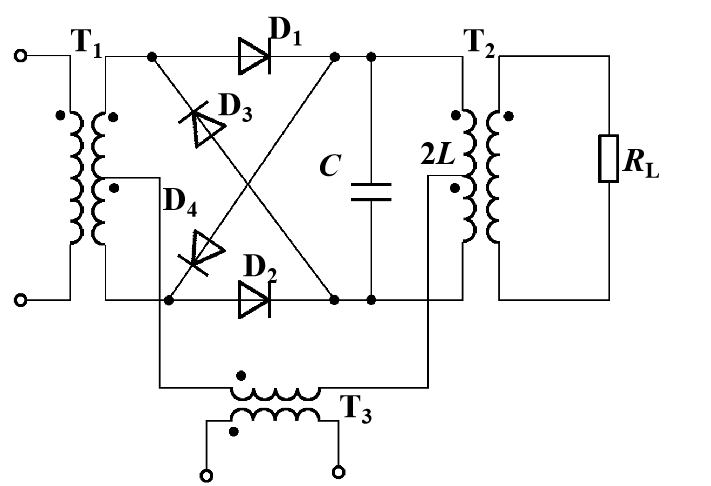
\includegraphics[scale=0.6]{image/Picture13.png}
    \caption{二极管环型调幅电路}
\end{figure}

\subsubsection{模拟乘法器调幅电路}

模拟乘法器有两个输入端 ( $X$ 输入和 $Y$ 输入) 和一个输出端,是一个三端口网络。

\begin{figure}[htbp]
    \centering
    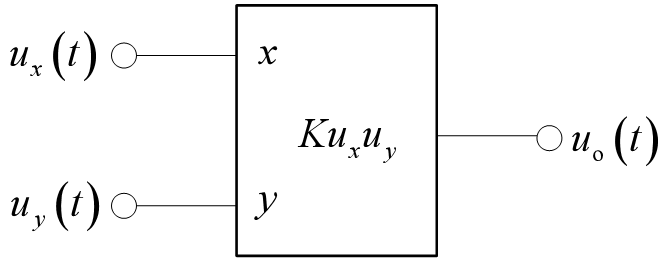
\includegraphics[scale=0.4]{image/Picture14.png}
    \caption{模拟乘法器调幅电路}
\end{figure}

理想的传输特性 (注意有时输出为电流):

\begin{equation}
    u_o(t) = K u_x(t) u_y(t)
\end{equation}

其中 $K$ 为增益系数或标度因子,单位为 1/V。

\subsection{高电平调幅电路}

高电平调幅电路通过丙类谐振功放实现;输出功率大、效率高、调制线性度好;用于产生普通调幅波。

\subsubsection{集电极调幅电路}

集电极调幅电路调制信号控制集电极电源电压,工作于过压区,效率高。

\begin{figure}[htbp]
    \centering
    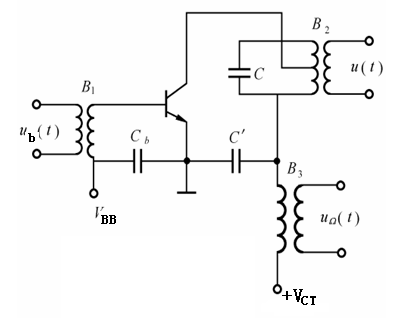
\includegraphics[scale=0.6]{image/Picture15.png}
    \caption{集电极调幅电路}
\end{figure}

集电极有效电源电压随调制信号变化,为:

\begin{equation}
    V_{CC} = V_{CT} + u_{\Omega}(t)
\end{equation}

在过压区,$I_{C0}$、$I_{c1m}$ 与 $V_{CC}$ 成线性关系。

$U_{\Omega m} = V_{CT}$ 时可达到 $100\%$ 调幅。

未调制时,其各功率和效率为:

\begin{equation}
\begin{aligned}
    P_{=T} &= V_{CC} I_{C00} = V_{CT} I_{COT} \\
    P_{oT} &= \frac{1}{2} I_{c1m}^2 R_p = \frac{1}{2} I_{C1T}^2 R_p \\
    P_{cT} &= P_{=T} - P_{oT} \\
    \eta_{cT} &= \frac{P_{oT}}{P_{=T}}
\end{aligned}
\end{equation}

在调制最高点的各功率都是载波状态对应功率的 $\left(1 + m_a\right)^2$ 倍。

在调制一周内的各平均功率都是载波状态对应功率的 $\left(1 + \frac{m_a^2}{2}\right)$ 倍。

集电极调幅调制过程中效率不变。

应采用管子的允许损耗功率 $P_{CM} > P_{\text{cav}}$。

\subsubsection{基极调幅电路}

基极调幅电路调制信号控制基极电源电压,工作于欠压区,效率较低,适用于小功率发射机。

\begin{figure}[htbp]
    \centering
    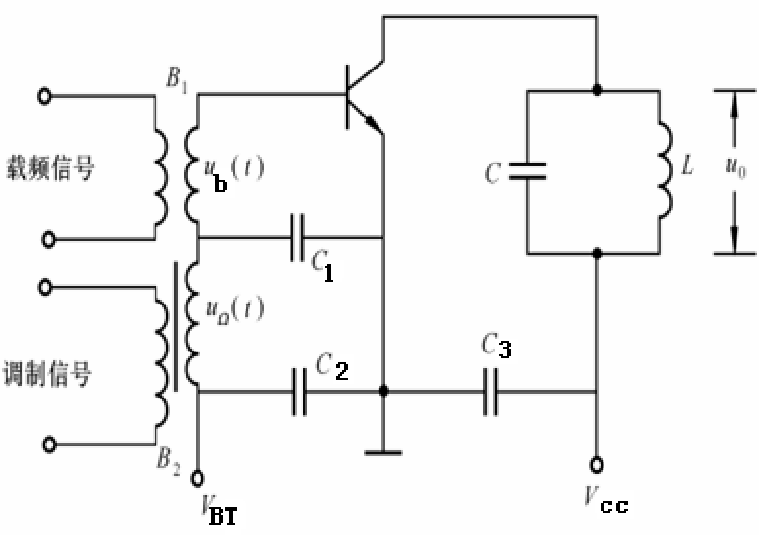
\includegraphics[scale=0.5]{image/Picture16.png}
    \caption{基极调幅电路}
\end{figure}

基极调幅电路的调幅度:

\begin{equation}
    m_a = \frac{U_{\Omega m}}{V_{BT}}
\end{equation}

基极调幅调制过程中效率是变化的;输入功率都由直流电源提供。

\section{调幅信号的解调}

\subsection{检波概述}

从频谱上看,检波是一种信号频谱的线性搬移过程,将调幅波的边频或边带频谱搬移到原调制信号的频谱处。

检波电路的分类:

(1) 包络检波:检波器的输出电压直接反映输入高频调幅波包络变化规律,只适合于普通调幅波的检波。

(2) 同步检波:在检波器的输入端加一个与本地载波信号同频同相的同步信号实现检波,主要用于DSB调幅波和SSB调幅波的检波。

\subsection{二极管大信号包络检波器}

二极管大信号包络检波器由输入回路、二极管 $D$ 和 $RC$ 低通滤波器组成。

\begin{figure}[htbp]
    \centering
    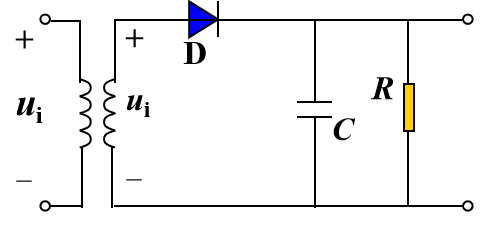
\includegraphics[scale=0.5]{image/Picture17.png}
    \caption{二极管大信号包络检波器}
\end{figure}

二极管大信号包络检波器的输出包括直流及低频调制分量。

电压传输系数 (检波效率) 定义为输出低频交流电压振幅与输入已调波包络振幅的比值,即:

\begin{equation}
    K_d = \frac{U_{\Omega m}}{m_a U_{im}}
\end{equation}

失真情况:

(1) 频率失真:电容 $C$ 和 $C_c$ 对不同的频率具有不同的容抗值。

(2) 非线性失真:二极管伏安特性起始弯曲部分引起的信号失真。

(3) 惰性失真:如果 $RC$ 取值过大,放电时间常数所对应的放电速度小于输入信号包络下降速度,输出波形不随输入信号包络而变化。

(4) 负峰切割失真:在输入调幅波包络的负半周峰值处可能会低于 $U_R$,使二极管截止,检波输出信号不跟随输入调幅波包络的变化。

\begin{figure}[htbp]
    \centering
    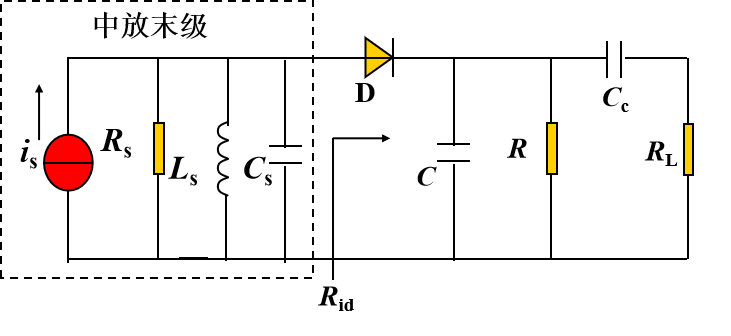
\includegraphics[scale=0.6]{image/Picture18.png}
    \caption{包络检波器的设计}
\end{figure}

检波器设计及元件参数的选择:

(1) 回路有载 $Q_L$ 要大:

\begin{equation}
    Q_L = \omega_c C_s (R_s // R_{id}) >> 1
\end{equation}

(2) 输出的高频纹波小:

\begin{equation}
    RC >> \frac{1}{\omega_c}
\end{equation}

(3) 避免频率失真:

\begin{equation}
    RC << \frac{1}{\Omega_{\text{max}}}, \quad R_L C_c >> \frac{1}{\Omega_{\text{min}}}
\end{equation}

(4) 避免惰性失真:

\begin{equation}
    RC \leq \frac{\sqrt{1 - m_a^2}}{\Omega_{\text{max}} m_a}
\end{equation}

(5) 避免底部切割失真:

\begin{equation}
    m_a < \frac{R_L}{R + R_L} \quad \text{or} \quad \frac{R_L // R}{R}
\end{equation}

\subsection{同步检波器}

同步:在输入端外加一个与原载频信号同频同相的本地载频信号。

若乘法器输出特性为电压,则:

输入为双边带或单边带调幅波时,输出:

\begin{equation}
    u_{\Omega} = \frac{1}{2} K U_{im} U_{0m} \cos{\Omega t}
\end{equation}

设本地载频信号与输入载频的不同步量为 $\Delta \omega$,相位不同步量为 $\varphi$,即:

\begin{equation}
    u_0 = U_{0m} \cos{[(\omega_c + \Delta \omega)t + \varphi]}
\end{equation}

输入为双边带调幅波,本地载频信号不同步时,输出:

\begin{equation}
    u_{\Omega} = \frac{1}{2} K U_{im} U_{0m} \cos{(\Delta \omega t + \varphi)} \cos{\Omega t}
\end{equation}

输入为单边带调幅波,本地载频信号不同步时,输出:

\begin{equation}
    u_{\Omega} = \frac{1}{2} K U_{im} U_{0m} \cos{\left[(\Omega - \Delta \omega)t - \varphi\right]}
\end{equation}

即当频率、相位不同步时,检出的低频信号将产生频率失真和相位失真。

